\documentclass[a4paper,12pt,oneside]{book}
\usepackage{polski}
\usepackage[utf8]{inputenc}
\usepackage{graphicx}
\graphicspath{{./images}}
\usepackage[shortlabels]{enumitem}
\usepackage{amssymb}
\usepackage{amsmath}
\usepackage{indentfirst}
\usepackage{pdfpages}

\usepackage{tikz}
%\usepackage{etoolbox} % for \ifthen
\usepackage{listofitems} % for \readlist to create arrays
\usetikzlibrary{arrows.meta} % for arrow size
\usepackage[outline]{contour} % glow around text
\contourlength{1.4pt}
\usepackage[margin=1in]{geometry}
\usepackage{listings}
\usepackage{booktabs}
\usepackage{tabularx}


\tikzset{>=latex} % for LaTeX arrow head
\usepackage{xcolor}
\colorlet{myred}{red!80!black}
\colorlet{myblue}{blue!80!black}
\colorlet{mygreen}{green!60!black}
\colorlet{myorange}{orange!70!red!60!black}
\colorlet{mydarkred}{red!30!black}
\colorlet{mydarkblue}{blue!40!black}
\colorlet{mydarkgreen}{green!30!black}
\tikzstyle{node}=[thick,circle,draw=myblue,minimum size=22,inner sep=0.5,outer sep=0.6]
\tikzstyle{node in}=[node,green!20!black,draw=mygreen!30!black,fill=mygreen!25]
\tikzstyle{node hidden}=[node,blue!20!black,draw=myblue!30!black,fill=myblue!20]
\tikzstyle{node convol}=[node,orange!20!black,draw=myorange!30!black,fill=myorange!20]
\tikzstyle{node out}=[node,red!20!black,draw=myred!30!black,fill=myred!20]
\tikzstyle{connect}=[thick,mydarkblue] %,line cap=round
\tikzstyle{connect arrow}=[-{Latex[length=4,width=3.5]},thick,mydarkblue,shorten <=0.5,shorten >=1]
\tikzset{ % node styles, numbered for easy mapping with \nstyle
	node 1/.style={node in},
	node 2/.style={node hidden},
	node 3/.style={node out},
}
\def\nstyle{int(\lay<\Nnodlen?min(2,\lay):3)} % map layer number onto 1, 2, or 3

\def\shrug{\texttt{\raisebox{0.75em}{\char`\_}\char`\\\char`\_\kern-0.5ex(\kern-0.25ex\raisebox{0.25ex}{\rotatebox{45}{\raisebox{-.75ex}"\kern-1.5ex\rotatebox{-90})}}\kern-0.5ex)\kern-0.5ex\char`\_/\raisebox{0.75em}{\char`\_}}}

\renewcommand\thechapter{\Roman{chapter}}
\renewcommand\thesection{\arabic{section}}
\renewcommand\thesubsection{\thesection.\arabic{subsection}}

\begin{document}

	
\includepdf{Odpowiedz-cover-page.pdf}

	\tableofcontents
	\newpage
	
	\chapter{Pytania - dr. hab. Grzegorz Wójcik}
	
		\section{Bazy danych}
			\subsection{Model relacyjny baz danych i języki zapytań.}
			
				\subsubsection{Model relacyjny baz danych}
				
				Relacyjny model danych pojawił się po raz pierwszy w artykule naukowym Edgara Codda w 1970 roku.
				W terminologii matematycznej - baza danych jest zbiorem relacji.  Stąd historycznie pochodzi nazwa relacyjny model danych i relacyjna baza danych. W matematyce definiuje się relację jako podzbiór iloczynu kartezjańskiego zbiorów wartości. Reprezentacją relacji jest dwuwymiarowa tabela złożona z kolumn i wierszy. \\ \\ Założenia modelu relacyjnego:
				\begin{itemize}
				\itemsep 0em
				\item Liczba \textbf{kolumn/atrybutów/pól (synonimy)} jest z góry ustalona.
				\item Z każdą kolumną jest związana jej nazwa (np. FirstName) oraz dziedzina (np. TEXT(20)), określająca zbiór wartości, jakie mogą wystąpić w kolumnie.
				\item Na przecięciu \textbf{wiersza/krotki/rekordu (synonimy)} i kolumny znajduje się pojedyncza (atomowa) wartość należąca do dziedziny kolumny.
				\item Wiersz reprezentuje jeden rekord informacji np. osobę.
				\item W modelu relacyjnym abstrahujemy od kolejności wierszy (rekordów) i kolumn (pól w rekordzie).
				\end{itemize}
				
				\noindent \textbf{Klucz główny}: dla każdej tabeli musi być określony klucz główny, będący jednoznacznym identyfikatorem. Może to być jedna lub więcej kolumn, w których wartości jednoznacznie identyfikują cały wiersz. Klucz główny w tabeli może być tylko jeden. \\
				\textbf{Klucz jednoznaczny} ma te same właściwości co klucz główny, ale ich może być w tabeli więcej niż jeden. \\
				\textbf{Klucz obcy} - jedna lub więcej kolumn, których wartości występują również jako klucz główny/jednoznaczny w tej samej/innej tabeli i są interpretowane jako wskaźniki do wierszy w tej drugiej tabeli
				
				\noindent \\ \textbf{Dwanaście postulatów Codda} – jest to zestaw 13 zasad stworzonych przez Edgara F. Codda – pioniera relacyjnych baz danych. Każda relacyjna baza danych musi je spełniać:
				\begin{itemize}
				\itemsep 0em
					\item System musi być kwalifikowany jako relacyjny, jako baza danych i jako system zarządzania.
					\item \textbf{Postulat informacyjny} – dane są reprezentowane jedynie przez wartości atrybutów w wierszach tabel (w krotkach).
					\item \textbf{Postulat dostępu} – każda wartość w bazie danych jest dostępna poprzez podanie nazwy tabeli, atrybutu i wartości klucza podstawowego (głównego).
					\item \textbf{Postulat dotyczący wartości NULL} – dostępna jest specjalna wartość NULL dla reprezentacji zarówno wartości nieokreślonej, jak i nieadekwatnej, inna od wszystkich i podlegająca przetwarzaniu.
					\item \textbf{Postulat dotyczący katalogu} – wymaga się, aby system obsługiwał wbudowany katalog relacyjny z bieżącym dostępem dla uprawnionych użytkowników używających języka zapytań.
					\item \textbf{Postulat języka danych} – system musi dostarczać pełny język przetwarzania danych, który może być używany zarówno w trybie interaktywnym, jak i w obrębie programów, obsługuje operacje definiowania danych, operacje manipulowania danymi, ograniczenia związane z bezpieczeństwem i integralnością oraz operacje zarządzania transakcji.
					\item \textbf{Postulat modyfikowalności perspektyw} – system musi umożliwiać modyfikowanie perspektyw, o ile jest ono semantycznie realizowalne.
					\item \textbf{Postulat modyfikowalności danych} – system musi umożliwiać operacje modyfikacji danych, musi obsługiwać operacje INSERT, UPDATE oraz DELETE.
					\item \textbf{Postulat fizycznej niezależności danych} – zmiany fizycznej reprezentacji danych i organizacji dostępu nie wpływają na aplikacje.
					\item \textbf{Postulat logicznej niezależności danych} – zmiany wartości w tabelach nie wpływają na aplikacje.
					\item \textbf{Postulat niezależności więzów spójności} – więzy spójności są definiowane w bazie i nie zależą od aplikacji.
					\item\textbf{ Postulat niezależności dystrybucyjnej} – działanie aplikacji nie zależy od modyfikacji  i dystrybucji bazy.
					\item \textbf{Postulat bezpieczeństwa względem operacji niskiego poziomu} – operacje niskiego poziomu nie mogą naruszać modelu relacyjnego i więzów spójności.
				\end{itemize}
				
			\noindent Operacje modelu relacyjnego:
			\begin{itemize}
				\itemsep 0em
				\item Selekcja - \verb*|WHERE| - selekcja podzbioru wierszy które spełniają określone warunki
				\item Projekcja - \verb*|SELECT| - pominięcie z wyniku pewnych kolumn
				\item Opracje na zbiorach: iloczyn kartezjański - \verb*|FROM| (złączenie tabel), suma zbiorów - \verb*|UNION|, różnica zbiorów - \verb*|EXCEPT|
				\item Agregacja - funkcje agregujące \verb*|SUM|, \verb*|MIN| itd. oraz klauzula \verb*|GROUP BY|
			\end{itemize}
			
			\newpage \subsubsection{Języki zapytań}
			\textbf{SQL} - Structured Query Language - jest to język strukturalny (i deklaratywny) służący do zarządzania bazą danych (CRUD). SQL jest najbardziej znanym językiem zapytań, ale istnieje także xBase.
			
			\begin{itemize}
			\item \textbf{DML (Data Manipulation Language)} służy do wykonywania operacji na danych – do ich umieszczania w bazie, kasowania, przeglądania oraz dokonywania zmian. Najważniejsze polecenia z tego zbioru to:
			\subitem \verb*|INSERT| – umieszczenie danych w bazie,
			\subitem \verb*|UPDATE| – zmiana danych,
			\subitem \verb*|DELETE| – usunięcie danych z bazy.
			
			\item \textbf{DDL (Data Definition Language)} - operacje na strukturach, w których dane są przechowywane – czyli np. dodawanie, zmienianie i kasowanie tabel lub baz. Najważniejsze polecenia tej grupy to:
			
			\subitem \verb*|CREATE| – utworzenie struktury (bazy, tabeli, indeksu itp.)
			\subitem \verb*|DROP| – usunięcie struktury
			\subitem \verb*|ALTER| – zmiana struktury

			\item \textbf{DCL (Data Control Language)} ma zastosowanie do nadawania uprawnień do obiektów bazodanowych. Najważniejsze polecenia w tej grupie to:
			
			\subitem \verb*|GRANT| – nadawanie uprawnień do pojedynczych obiektów lub globalnie konkretnemu użytkownikowi
			\subitem \verb*|REVOKE| – odbieranie wskazanych uprawnień konkretnemu użytkownikowi
			\subitem \verb*|DENY| – zabranianie wykonywania operacji

			\item \textbf{DQL (Data Query Language}) to język formułowania zapytań do bazy danych. W zakres tego języka wchodzi jedno polecenie – \verb*|SELECT|. Często SELECT traktuje się jako część języka DML, ale to podejście nie wydaje się właściwe, ponieważ DML z definicji służy do manipulowania danymi – ich tworzenia, usuwania i uaktualniania. Na pograniczu obu języków znajduje się polecenie SELECT INTO, które dodatkowo modyfikuje (przepisuje, tworzy) dane.
			\end{itemize}
				
				
			\newpage\subsection{Model obiektowo-relacyjny baz danych, inne modele danych.}
			\subsubsection{Model relacyjny}
			W relacyjnym modelu baz danych informacja jest zapisywana w tabeli w formie wierszy. Tabele tworzą między sobą powiązania zwane relacjami. Dużo dużo więcej jest napisane podrozdział wyżej
			
			\subsubsection{Model obiektowy}
			Model obiektowy łączy cechy programów komputerowych tworzonych w językach programowania obiektowego z cechami aplikacji bazodanowych. Obiekt w bazie reprezentuje obiekt w święcie rzeczywistym. Występują tutaj pojęcia klasa, obiekt, dziedziczenie, hermetyzacja. 
			\begin{itemize}
			\itemsep 0em
			\item oprócz danych dostępne są także operacje na danych
			\item użytkownik może definiować własne typy danych
			\item aplikacja oraz BD może być tworzona przy pomocy jednego języka
			\item aplikacja korzystająca z bazy nie wymaga zmiany modelu relacyjnego na obiektowy
			\item nie występuje problem z optymalizacją zapytań
			\item nie występuje ujednolicony standard modelu obiektowego
			\end{itemize}
			
			\subsubsection{Model obiektowo-relacyjny}
			Model ten łączy koncepcję modelu relacyjnego oraz obiektowego. Jego ideą jest połączenie najlepszych cech obydwu modeli.
			\begin{itemize}
				\itemsep 0em
				\item występują tutaj tabele które mogą mieć pola o typie ATD (Abstract Data Type). Umożliwiają one przechowywanie w bazie np. list, kolejek, drzew - obiektów którym możemy przypisać pewne cechy i zachowanie - mają swoje własne implementacje sortowania, wyszukiwania itp
				\item przystosowanie do przechowywania multimediów
				\item ten model zwraca dane jako tabele krotek (jak w bazie relacyjnej), a nie jako kolekcję
				obiektów
				\item programista musi zamienić odpowiedź z bazy danych będącą w postaci krotek (jak w
				relacyjnej) na postać obiektową
			\end{itemize}
			
			\subsubsection{Model hierarchiczny}
			W tym modelu przechowywane dane są zorganizowane w postaci drzewa. Informacja jest zawarta w dokumentach oraz w strukturze drzewa (podobnej do drzewa folderów na dysku komputera).
			\begin{figure}[h]
				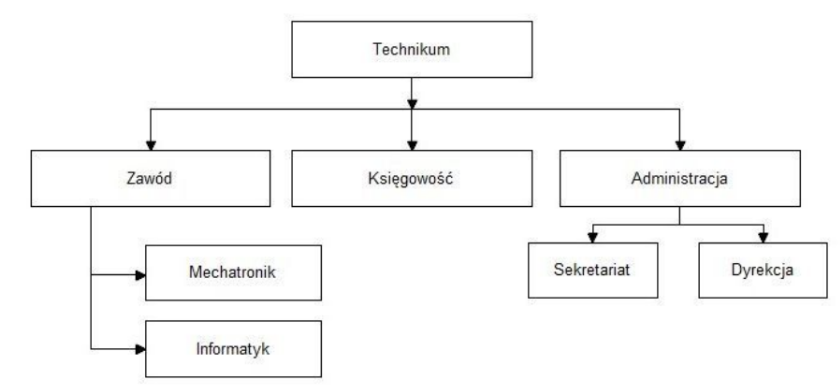
\includegraphics[width=10cm]{modelhierarchiczny}
				\centering
			\end{figure}
			\begin{itemize}
				\itemsep 0em
				\item dane są przedstawione w postaci drzewa (najłatwiej to porównać do XML)
				\item informacje są przechowywane w strukturze drzewa
				\item tabele muszą być zawsze ze sobą powiązane, czyli podrzędne z nadrzędnym (np.
				uczeń musi być podpięty pod jakąś szkołę)
				\item usunięcie tabeli nadrzędnej powoduje usunięcie wszystkich tabel podrzędnych
			\end{itemize}
			\subsubsection{Model sieciowy}
			Połączenia między dokumentami tworzą sieć. Informacja jest zawarta w dokumentach oraz w przebiegu połączeń sieci.
			\begin{figure}[h]
				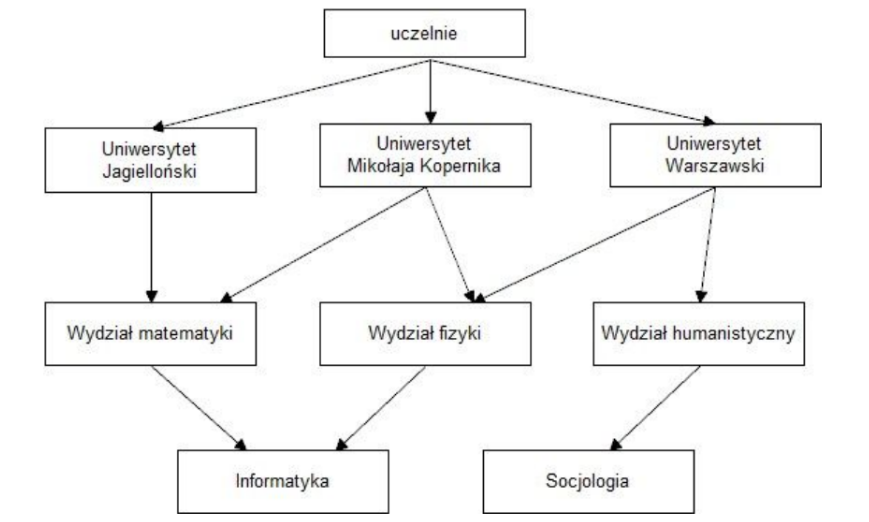
\includegraphics[width=10cm]{modelsieciowy}
				\centering
			\end{figure}
			\begin{itemize}
				\itemsep 0em
				\item jest to rozwinięcie modelu hierarchicznego gdzie tabele podrzędne mają wiele tabel
				nadrzędnych (skutkiem czego jest stworzenie grafu/sieci)
				\item można bezpośrednio odczytywać każdą tabele (nie trzeba przechodzić od korzenia
				do liścia jak w hierarchicznym)
				\item relacje/zależności między tabelami są nazywane strukturami
				\item w strukturze można wyłonić jedną tabelę główną z której to można przejść do tabel
				podrzędnych
				\item struktura jest relacja 1:N
				\item zmiany w bazie są bardzo trudne do wykonania
			\end{itemize}
			\subsubsection{Model semistrukturalny}
			\begin{itemize}
				\itemsep 0em
				\item polega na przedstawieniu danych w postaci modelu XML		
				\item przedstawia on dane w postaci drzewiastej (czyli jest hierarchiczny)
				\item zapytania są w postaci ścieżki
				\item atrybuty znacznika przechowywują dodatkowe informacje (cechy)
				\item dane w postaci XML można łatwo umieścić na stronie WWW (tylko trzeba określić sposób wyświetlania)
				\item baza w postaci /xML może być łatwo przekonwertowana na obiekt
			\end{itemize}
			
			\subsubsection{Model jednorodny}
			Wszystkie dane upchane w jednej tabeli, łatwo szukać danych po unikalnej wartości (ale ciężej po czymś nieunikalnym np nazwisko), taka forma posiada dużo duplikatów
				
			\newpage\subsection{Składnia podstawowych zapytań języka SQL.}
				\subsubsection{DDL - Data Definition Language}
				\noindent Jak zapamiętać skrót: \\ Definition = DEFINIOWANIE - TWORZENIE STRUKTUR \\
				\noindent W skład DDL wchodzą \verb*|DROP|, \verb*|CREATE| oraz \verb*|ALTER|.
				\begin{itemize}
					\itemsep 0em
					\item \verb*|DROP| - usunięcie struktury
					\begin{verbatim}
						DROP TABLE tabela;
					\end{verbatim}
					\item \verb*|CREATE| - stworzenie struktury
					\begin{verbatim}
						CREATE TABLE tabela(
							kolumna1 typ (rozmiar),
							kolumna2 typ (rozmiar),
							...
						);
					\end{verbatim}
					\item \verb*|ALTER| - modyfikacja struktury. Obejmuje operacje takie jak np. dodanie kolumny do tabeli, zmiana typu danych w kolumnie, usunięcie kolumny.
					\begin{verbatim}
						ALTER TABLE table
						ADD kolumna typ(dlugosc);
					\end{verbatim}
					\begin{verbatim}
						
					\end{verbatim}
				\end{itemize}
				
				
				\subsubsection{DML - Data Manipulation Language}
				\noindent Jak zapamiętać skrót: \\ Manipulation = MANIPULACJA - EDYCJA LUB TWORZENIE REKORDÓW \\
				\noindent W skład DML wchodzą \verb*|INSERT|, \verb*|UPDATE| oraz \verb*|DELETE|.
				\begin{itemize}
					\itemsep 0em
					\item \verb*|INSERT| - dodawanie wierszy
					\begin{verbatim}
						INSERT INTO tabela (kolumna1, kolumna2, ..., kolumna_n)
						VALUES (wartosc1, wartosc2, ..., wartosc_n)
					\end{verbatim}
					Nie trzeba podawać kolumn po nazwie tabeli gdy podamy po pierwsze wszystkie wartości, a po drugie w dobrej kolejności
					
					\item \verb*|UPDATE| - aktualizowanie danych, zmiana
					\begin{verbatim}
						UPDATE tabela
						SET kolumna1 = wartosc, kolumna2 = wartosc2, ...
						WHERE warunek
					\end{verbatim}
					WHERE nie jest konieczny, możemy  go użyć jak chcemy doprecyzować które rekordy mają się zaktualizować
					
					\item \verb*|DELETE| - usuwanie wierszy
					\begin{verbatim}
						DELETE FROM tabela
						WHERE warunek
					\end{verbatim}
					WHERE nie jest konieczny, możemy  go użyć jak chcemy doprecyzować które rekordy mają się skasować
				\end{itemize}
				\subsubsection{DCL - Data Control Language}
				\noindent Jak zapamiętać skrót: \\ Control = KONTROLA = UPRAWNIENIA \\
				\noindent W skład DCL wchodzą \verb*|GRANT|, \verb*|REVOKE| oraz \verb*|DENY|.
				
				\begin{itemize}
					\item \verb*|GRANT| - nadawanie uprawnień do pojedynczych obiektów lub globalnie konkretnemu userowi
					\item \verb*|REVOKE| - odbieranie uprawnień konkretnemu userowi
					\item \verb*|DENY| - zabranianie wykonywania operacji
					\item Składnia jest taka sama dla w/w poleceń:
					\begin{verbatim}
						[GRANT/REVOKE/DENY] operacja1, operacja2, ...
						ON tabela
						TO user
					\end{verbatim}
					Przykład:
					\begin{verbatim}
					GRANT SELECT, INSERT
					ON Fragment
					TO glazik
					\end{verbatim}
				\end{itemize}
				
				\subsubsection{DQL - Data Query Language}
				\noindent Jak zapamiętać skrót: \\ Query = ZAPYTANIA = SELECTY \\
				\noindent W skład DQL wchodzi jedno polecenie: \verb*|SELECT|. Pozwala wybierać wiersze z bazy danych. Składnia:
				\begin{verbatim}
					SELECT kolumny 
					FROM tabele 
					WHERE warunek
					GROUP BY kolumna
					HAVING warunek
					ORDER BY ... DESC/ASC;
				\end{verbatim}
				Dodatkowe klauzule \verb*|SELECT|:
				\begin{itemize}
					\itemsep 0em
					\item \verb*|ORDER BY| - sortowanie wyników względem np. kolumny
					\item \verb*|ASC| oraz \verb*|DESC| - dodawane po sortowaniu, wybieramy czy ma być ascending czy descending
					\item \verb*|GROUP BY| - grupowanie wyników względem danej kolumny
					\item \verb*|HAVING| - filtrowanie grup, działa podobnie do WHERE. WHERE oraz HAVING mogą występować jednocześnie w zapytaniu.
				\end{itemize}
				
			\newpage\subsection{Projektowanie baz danych oraz model związków encji.}
			\subsubsection{Projektowanie baz danych}
				Etapy projektowania systemów bazodanowych:
				\begin{itemize}
					\item \textbf{Sformułowanie problemu}
					\item \textbf{Analiza wycinka rzeczywistości} - wywiad z ekspertem dziedzinowym, analiza wymagań funkcjonalnych (co dodawać, co usuwać itd.) i niefunkcjonalnych (tryb graficzny, platforma sprzętowa itd.)
					\item \textbf{Opracowanie konceptualnego modelu danych}, czyli wyodrębnienie i zdefiniowanie encji, związków między nimi oraz atrybutów (taka jakby luźna forma) \\
					Projektowanie modelu konceptualnego bazy danych składa się z następujących etapów:
					\begin{itemize}
						\item \textbf{określenie zbiorów encji} - jakie encje (tabele) będzie zawierać baza?
						\item \textbf{określenie atrybutów encji} - jakie cechy (kolumny) będą miały poszczególne encje?
						\item \textbf{określenie dziedziny atrybutów} - jaki zakres wartości będzie miał każdy atrybut?
						\item \textbf{ustalenie kluczy podstawowych} - a'la klucze główne (?)
						\item \textbf{określenie związków między encjami} - a'la klucze obce (?)
					\end{itemize}
					\textbf{Encja} to każdy element rzeczywistości, który można scharakteryzować i odróżnić od innych obiektów, np. książka (przedmiot), klient (obiekt), zamówienie (zjawisko), stan cywilny (stan). \\
					\textbf{Atrybut} to cecha encji. Zestaw atrybutów, które określamy dla encji, zależy od potrzeb bazy danych (np. książka ma atrybuty: tytuł, autor, ...) \\
					\textbf{Dziedzina} opisuje jakie wartości może przyjąć dany atrybut, np. tytuł książki to napis o długości do x znaków.
					\item \textbf{Opracowanie modelu logicznego}, czyli wyrażenie świata rzeczywistego za pomocą reguł modelu danych (np. relacyjnego). Transformujemy model konceptualny do logicznego. Zamiast encji są tabele, zamiast związków są wiązania poprzez klucze główne i obce itd. Następuje normalizacja relacji.
					\item \textbf{Opracowanie modelu fizycznego}, czyli konstruowanie modelu świata rzeczywistego za pomocą struktur danych i mechanizmów istniejących w wybranym SZBD (systemie zarządzania bazami danych), czyli np naklepanie tego w MySQL
					\item \textbf{Tworzenie aplikacji}
					\item \textbf{Testowanie systemu}
				\end{itemize}
				
			\newpage
			\subsubsection{Model związków encji}
			\noindent  Model związków encji (model ER lub ERD) to jedna z najpopularniejszych metod modelowania danych. Służy do graficznego przedstawiania koncepcji projektowanej bazy danych. Jest bardzo podobny do relacyjnego modelu. Diagram taki pokazuje obiekty (encje), ich cechy (atrybuty) oraz relacje między nimi. Elementy takie, jak encja, atrybut oraz związek zostały opisane stronę wyżej. \\ \\
			Typy związków encji:
			\begin{itemize}
				\itemsep 0em
				\item \textbf{jeden do jednego} (1:1) \\
				Związek ten określa, iż każde wystąpienie danego obiektu (encji) związane jest wyłącznie z pojedynczym wystąpieniem innego bytu. Na przykład: Pracownik w organizacji ma przypisane konkretne Miejsce, a to Miejsce jest przypisane do konkretnego Pracownika. Kierownik zarządza jednym Działem, a Dział zarządzany jest przez jednego Kierownika.
				\item \textbf{jeden do wielu} (1:N) \\
				Związek ten określa, iż jedno wystąpienie danego obiektu (encji) związane jest z większą ilością wystąpień innego bytu. Na przykład: Klient składa wiele Zamówień. Konkretne Zamówienie jest składane przez danego Klienta. W Firmie istnieje wiele Działów. Konkretny Dział istnieje w danej Firmie.
				\item \textbf{wiele do wielu} (M:N) \\
				Związek ten określa, iż jedno wystąpienie danego obiektu (encji) związane jest z większą ilością wystąpień innego bytu, tak samo jak jedno wystąpienie innego bytu może być powiązane z większą ilością wystąpień tego pierwszego obiektu. Przykładem takiego związku może być zależność jaka występuje pomiędzy Studentem oraz Wykładem. Student zapisany może być na wiele Wykładów, tak i na dany Wykład zapisanych może być wielu Studentów.
			\end{itemize}
			
			\newpage\subsection{Problemy indeksowania baz danych, rodzaje indeksów, indeksy typu B+ drzewo.}
				\subsubsection{Problemy indeksowania baz danych}
				Problem z przeszukiwaniem baz danych polega na tym, że… tabele w MySQL (a także w innych RDBMS) \textbf{nie są posortowane według kolumn}, dzięki którym wyciągamy odpowiednie dane. Dane ulegają aktualizacji, usuwaniu i ciągle dodawane są nowe. Jedyna „kolejność” to często klucz główny, który jest de facto indeksem. Nie jest to przydatna kolejność kiedy szukamy danych nie po kluczu a po jakimś innym polu np:
					\begin{verbatim}
						SELECT nazwa_produktu FROM produkty WHERE cena = 128; 
					\end{verbatim}
				Jeżeli mielibyśmy te nasze produkty posortowane według ceny, to znalezienie było by banalne. W przypadku kiedy dane są posortowane po kluczu głównym trzeba „sprawdzić” wszystkie rekordy i nie mamy możliwości ułatwienia sobie zadania bo produkty mogą mieć przecież różną cenę. Mówi wtedy że dokonujemy \textbf{pełnego skanu tabeli} (ang. full table scan), który działa niekorzystnie na wydajność – zabiera po prostu za wiele czasu. Sztuka optymalizacji za pomocą indeksowania polega na unikaniu tego pełnego skanu. Działanie indeksu polega na tym, że zawiera w przystępnej postaci informację, w których komórkach pamięci znajdują się produkty o cenie 128. Z tego korzysta RDBMS – najpierw uderza do indeksu a kiedy już wie skąd ma pobrać dane to od razu przechodzi do odpowiednich miejsc bez przeszukiwania całej tabeli i zwraca wynik użytkownikowi. \\
				
				\noindent \textbf{Zalety indeksów:} znacznie przyspieszają pewne SELECTy \\
				\textbf{Wady selectów:} spowalniają dodawanie, modyfikowanie i usuwanie danych (w przypadku edycji tabeli należy również zaktualizować jej indeks)
				
				\subsubsection{Rodzaje indeksów}
				\begin{itemize}
					\item \textbf{Ze względu na liczbę wskazań indeksu (ile rekordów wskazuje indeks)}:
						\subitem \textit{indeks rzadki} - zawiera rekordy tylko dla wybranych rekordów indeksowanego pliku (indeksowana jest tylko część pliku)
						\subitem \textit{indeks gęsty} - zawiera rekord indeksu dla każdego rekordu indeksowanego pliku (indeksowany jest cały plik)
					\item \textbf{Ze względu na liczbę poziomów indeksu (indeks może wskazywać na inny indeks)}:
						\subitem \textit{indeks jednopoziomowy} - do pliku z danymi tworzony jest tylko jeden indeks na dany atrybut
						\subitem \textit{indeks wielopoziomowy} - do pliku z danymi tworzonych jest wiele indeksów na dany atrybut (tworzenie indeksu do indeksu)
					\item \textbf{Ze względu na charakterystykę indeksowanego atrybutu}:
						\subitem \textit{indeks podstawowy} - - jest on założony na atrybucie (unikalnym) który umożliwia porządkowanie pliku (np. klucz główny, PESEL, dane osobowe). Jest to indeks rzadki.
						\subitem \textit{indeks zgrupowany} - jest on zakładany na atrybucie który nie jest unikalny (również umożliwia porządkowanie pliku) (np. imię, wartość liczbowa). Ten indeks wskazuje na pierwszy blok w którym występuje dana wartość (patrz wartość 2, 3, 4). Jest to indeks rzadki.
						\subitem \textit{indeks wtórny} - jest on zakładany na atrybucie który nie jest atrybutem uporządkowanym (czyli taki według którego plik nie jest uporządkowany). Jest to indeks gęsty.
					\item \textbf{Ze względu na liczbę indeksowanych atrybutów}
						\subitem \textit{indeks z kluczem prostym} - indeksowany jest tylko jeden atrybut/klucz
						\subitem \textit{indeks z kluczem złożonym} - indeksowane jest wiele atrybutów jednocześnie (klucz)
					\item \textbf{Ze względu na zarządzanie strukturą}
						\subitem \textit{indeksowanie statyczne} - indeks nie ma mechanizmów które modyfikują strukturę czyli np. usuwanie pozostawia puste rekordy w indeksie, a dodawanie polega na dodawaniu rekordów do specjalnego miejsca zwanego “blokiem przepełnienia”
						\subitem \textit{indeksowanie dynamiczne} - indeks ma mechanizmy które modyfikują strukturę (i nie ma tych problemów co w indeksowaniu statycznym)
				\end{itemize}
				\subsubsection{Indeksy typu B+ drzewo}
				\begin{itemize}
				\itemsep 0em
				\item to rodzaj indeksowania dynamicznego wielowarstwowego które jest przedstawione w postaci drzewa
				\item każdy indeks posiada wskaźnik (który nie jest liściem) wskazuje na inny indeks
				\item wskaźnik po lewej stronie klucza (wartości atrybutu) zawiera wartości mniejsze, a po prawej większe
				\item węzły tego drzewa mogą pomieścić określona ilość rekordów indeksu
				\item gdy rekordów w węźle jest za dużo to następuje dzielenie węzła, a gdy w dwóch węzłach jest mniej niż połowa to następuje łączenie węzłów
				\item B+ drzewo rośnie do góry (tak samo jak B)
				\item jest to drzewo zrównoważone (odległość od korzenia do liścia wszędzie jest taka sama)
				\item węzły które nie są liśćmi nie posiadają wartości (w B-drzewie posiadały)
				\item wartości kluczy które są w węzłach wewnętrznych powtarzają się w liściach (np. (2,4) C (1,2,3,4,5)
				\item liście są ze sobą połączone (liść o mniejszych wartościach ma wskaźnik do liścia o większych wartościach)
				\item Wyszukiwanie informacji w drzewie wynosi O(logn)
				\end{itemize}

			\newpage\subsection{Przetwarzanie transakcyjne OLTP (On-Line Transaction Processing).}
		\textbf{OLTP} (Online Transaction Processing) to kategoria aplikacji klient-serwer dotyczących baz danych w ramach bieżącego przetwarzania transakcji obejmujących takie zastosowania jak systemy rezerwacji, obsługa punktów sprzedaży, systemy śledzące itp. W systemach tych klient współpracuje z serwerem transakcji, zamiast z serwerem bazy danych.  Zastosowanie - np. w bankowości internetowej, w handlu detalicznym, podczas składania zamówień lub przy wysyłaniu wiadomości tekstowych. Transakcje te (tradycyjnie określane jako transakcje gospodarcze lub finansowe) są rejestrowane i zabezpieczane w taki sposób, aby przedsiębiorstwo mogło w każdej chwili uzyskać do nich dostęp w celach księgowych lub sprawozdawczych. \\

		System OLTP:
		\begin{itemize}
			\itemsep 0em
			\item Umożliwia wykonywanie w czasie rzeczywistym dużej liczby transakcji bazodanowych przez dużą liczbę osób
			\item Wymaga błyskawicznych czasów reakcji
			\item Często modyfikuje małe ilości danych i zazwyczaj dokonuje tyle samo odczytów, co zapisów danych
			\item Używa indeksowanych danych w celu skrócenia czasu odpowiedzi
			\item Wymaga częstego lub równoczesnego wykonywania kopii zapasowych bazy danych
			\item Wymaga stosunkowo niewiele miejsca do przechowywania danych
			\item Zazwyczaj obsługuje proste zapytania dotyczące tylko jednego lub kilku rekordów
		\end{itemize}
		
		\textbf{Transakcja} to zbiór operacji na bazie danych, które stanowią w istocie pewną całość i powinny być wykonane wszystkie lub żadna z nich. Składa się zawsze z trzech etapów: \textbf{rozpoczęcia, wykonania i zamknięcia}. W systemach bazodanowych istotne jest, aby trwała jak najkrócej, ponieważ równolegle może być wykonywane wiele transakcji i część operacji musi zostać wykonana w pewnej kolejności. Każdy etap transakcji jest logowany, dzięki czemu w razie awarii można odtworzyć stan bazy sprzed transakcji. \\
		Cechy transakcji: \textbf{ACID} \\
		- \textbf{A}tomicity - atomowość - wykona się wszystko albo nic (zbiór operacji = całość); \\
		- \textbf{C}onsistency - spójność - baza przed i po zmianach jest spójna; \\
		- \textbf{I}solation - izolacja - równolegle wykonywane transakcje nie mają na siebie wpływu; \\
		- \textbf{D}urability - trwałość - zmiany prowadzone przez transakcje są trwałe (nawet w przypadku awarii);\\
		W SQL wyróżniamy następujące polecenia dotyczące transakcji:
		\begin{itemize}
			\itemsep 0em
			\item \verb*|BEGIN| lub \verb*|BEGIN WORK| – rozpoczęcie transakcji
			\item \verb*|COMMIT| – zatwierdzenie zmian wykonanych w obrębie transakcji
			\item \verb*|ROLLBACK| – odrzucenie zmian wykonanych w obrębie transakcji
			\item \verb*|SAVEPOINT nazwa| – zdefiniowanie punktu pośredniego o określonej nazwie
			\item \verb*|RELEASE SAVEPOINT nazwa| – skasowanie punktu pośredniego (nie wpływa w żaden sposób na stan transakcji)
			\item \verb*|ROLLBACK TO SAVEPOINT nazwa| – wycofanie transakcji do stanu zapamiętanego w podanym punkcie pośrednim.
		\end{itemize}
		\newpage\section{Paradygmaty}
			\subsection{Założenia paradygmatu programowania obiektowego.}
				Paradygmat obiektowy zakłada modułowość, czyli tworzenie programu z wcześniej
				zdefiniowanych komponentów (np. klasy).
				
				Główne założenia paradygmatu programowania obiektowego:
				\begin{enumerate}
					\item \textbf{Abstrakcja} - to przedstawienie obiektu ze świata rzeczywistego i jego cech jako
					uproszczony model/szablon (tutaj klasa i obiekty) wykorzystywany w problemie
					programistycznym.
					\item \textbf{Hermetyzacja (enkapsulacja)} - to ukrycie implementacji przed użytkownikiem
					(prywatne pola - publiczne metody).
					Cytując kogoś mądrego: “Hermetyzacja polega na tym, że klasy są zamkniętymi
					"czarnymi skrzynkami" - inne klasy nie muszą wiedzieć dokładnie co się dzieje w
					środku, mogą wchodzić z nimi w interakcje poprzez elementy, które wystawiają
					publicznie (publiczne pola i metody)”.
					\item \textbf{Dziedziczenie} - jest to tworzenie hierarchii klas. Klasa dziedzicząca otrzymuje pola i
					metody (te może zmieniać) “klasy matki”. Tworzenie bardziej wyspecjalizowanego
					obiektu z bardziej ogólnego. (np. klasa jabłko dziedziczy cechy po klasie owoc)
					\item \textbf{Polimorfizm} - polega na dostosowaniu zachowania obiektów do oczekiwań
					użytkownika. Inaczej mówiąc gdy grupa obiektów dziedziczy metodę od innej klasy.
					Każda klasa która odziedziczyła tę metodę to ją zmieniła. Wywołanie tej
					odziedziczonej metody na poszczególnych obiektach wywoła wykonanie instrukcji
					zaimplementowanych dla każdego obiektu. (np. dla każdej figury funkcja obliczania
					pola będzie inna)
				\end{enumerate}
			\newpage\subsection{Idea dziedziczenia i polimorfizmu w programowaniu.}
				\subparagraph{Dziedziczenie} - jest to tworzenie hierarchii klas. Klasa dziedzicząca otrzymuje pola i metody
				(te może zmieniać) “klasy matki”. Tworzenie bardziej wyspecjalizowanego obiektu z bardziej
				ogólnego. (np. klasa jabłko dziedziczy cechy po klasie owoc).
				Umożliwia ona większą czytelność kodu który jednocześnie staje się prostszy (bo po co
				pisać 2 razy to samo)
				
				\subparagraph{Polimorfizm} - polega na dostosowaniu zachowania obiektów do oczekiwań użytkownika.
				Inaczej mówiąc gdy grupa obiektów dziedziczy metodę od innej klasy. Każda klasa która
				odziedziczyła tę metodę to ją zmieniła. Wywołanie tej odziedziczonej metody na
				poszczególnych obiektach wywoła wykonanie instrukcji zaimplementowanych dla każdego
				obiektu. (np. dla każdej figury funkcja obliczania pola będzie inna)
				
				Polimorfizm umożliwia nie tylko wykonywanie odpowiednio metod dla obiektów pochodnych
				ale również przypisanie do bardziej ogólnego typu danych (np. Owoc jablko= new Jablko(); )
			\newpage\subsection{Zasady programowania dynamicznego.}
				\subparagraph{Programowanie dynamiczne} - jest to rozszerzenie strategii "dziel i zwyciężaj". „Programowanie” oznacza w tym
				kontekście tabelaryczną metodę rozwiązywania problemów, a nie pisanie programów komputerowych. Wiemy, że w algorytmach typu „dziel i zwyciężaj” dzieli się problem na niezależne podproblemy, rozwiązuje je rekurencyjnie, a następnie łączy się rozwiązania
				wszystkich podproblemów w celu utworzenia rozwiązania pierwotnego problemu. Programowanie dynamiczne można stosować wtedy, kiedy podproblemy nie są niezależne, tzn. kiedy podproblemy mogą zawierać te same podpodproblemy. Wtedy algorytm typu „dziel i zwyciężaj” wykonuje więcej pracy niż to w istocie jest konieczne, wielokrotnie
				bowiem rozwiązuje ten sam podproblem. \\
				
				\begin{figure}[h!]
					\centering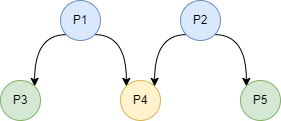
\includegraphics[scale=0.45]{problem_dynam.png}
					\caption{Przykładowy problem złożony}
				\end{figure}
				
				Jak widać na obrazku wyżej chcąc obliczyć rozwiązania problemów P1 i P2 rozwiązaniem typu "dziel i zwyciężaj", problem P4 zostałby policzony 2 razy jako problem zależny. Programowanie dynamiczne ma na celu optymalizację takich przypadków i pisząc program zapamiętalibyśmy rozwiązanie P4 gdy liczymy P1. Nastepnie obliczając drugi głowny problem - P2, znamy już rozwiązanie P4 więc nie marnujemy czasu i mocy obliczeniowej.\\
				
				\textbf{Proces projektowania algorytmu} opartego na programowaniu dynamicznym można podzielić na cztery etapy: 
				\begin{enumerate}
					\item Scharakteryzowanie struktury optymalnego rozwiązania. 
					\item Rekurencyjne zdefiniowanie kosztu optymalnego rozwiązania.
					\item Obliczenie optymalnego kosztu metodą wstępującą (ang. bottom-up) – czyli rozpoczynając od najmniejszych podproblemów, rozwiązywać coraz większe, wykorzystując zapamiętane rozwiązania mniejszych.
					\item Konstruowanie optymalnego rozwiązania na podstawie wyników wcześniejszych obliczeń. 
				\end{enumerate}
				
				\textbf{Zasady} paradygmatu programowania dynamicznego (pretty much to samo co proces projektowania) to:
				\begin{itemize}
					\item Scharakteryzować strukturę rozwiązania optymalnego.
					\item Zdefiniować rekurencyjnie wartość rozwiązania optymalnego, jako funkcję rozwiązań optymalnych dla podproblemów.
					\item Skonstruować optymalne rozwiązanie problemu na bazie wyliczonych wcześniej wielkości.
				\end{itemize}
			
			\newpage\subsection{Główne paradygmaty programowania.}
				\subparagraph{Paradygmat programowania} - jest to wzorzec sposobu programowania, patrzenia na dane,
				przepływ danych oraz sposób wykonywania programu.
				
				\subsubsection{Programowanie imperatywne}
				Chcąc najkrócej scharakteryzować programowanie imperatywne, moglibyśmy napisać „zrób najpierw to, a potem tamto”. Mamy zatem sekwencję poleceń zmieniających krok po kroku stan maszyny, aż do uzyskania oczekiwanego wyniku — czyli mamy stan będący funkcją czasu. Ten sposób patrzenia na programy związany jest ściśle z budową sprzętu komputerowego o architekturze von Neumanna, w którym poszczególne instrukcje to właśnie polecenia zmieniające ów globalny stan.
				
				Imperatywne języki programowania posługują się abstrakcjami bliskimi architekturze von Neumanna, np. zmienne są abstrakcją komórek pamięci. Naturalną abstrakcją są tu też procedury (będące, notabene, zasadniczym elementem „podparadygmatu” proceduralnego). Najważniejsze — w swoim czasie — języki imperatywne to Fortran, Cobol, Pascal i C.
				
				\subsubsection{Programowanie proceduralne}
				Programowanie proceduralne – paradygmat programowania zalecający dzielenie kodu na procedury, czyli fragmenty wykonujące ściśle określone operacje. Procedury nie powinny korzystać ze zmiennych globalnych (w miarę możliwości), lecz pobierać i przekazywać wszystkie dane (czy też wskaźniki do nich) jako parametry wywołania.
				
				\subsubsection{Programowanie strukturalne}
				O programowaniu strukturalnym wspominamy z kronikarskiego obowiązku, jest to bowiem bardzo dobrze znany i powszechnie stosowany „podparadygmat” programowania imperatywnego, czy ściślej — proceduralnego. Chodzi w nim o tworzenie programów z kilku dobrze zdefiniowanych konstrukcji takich jak instrukcja warunkowa if-then-else i pętla while, za to bez skoków (go to). Powinno to sprzyjać pisaniu programów przejrzystych, łatwych w rozumieniu i utrzymaniu.
				
				Ściślej, Dijkstra proponował użycie tylko trzech rodzajów struktur sterujących:
				\begin{itemize}
					\item Sekwencja (lub konkatenacja) — czyli po prostu wykonanie instrukcji w określonej kolejności. W wielu językach rolę „operatora konkatenacji instrukcji” spełnia niepozorny średnik...
					\item Wybór — czyli wykonanie jednej z kilku instrukcji zależnie od stanu programu. Przykładem jest if-then-else i switch/case.
					\item Iteracja, czyli powtarzanie instrukcji tak długo, jak długo spełniony (lub niespełniony) jest dany warunek. Chodzi oczywiście o pętle, np. while, repeat-until, for itp.
				\end{itemize}
			
			
				\subsubsection{Programowanie obiektowe}
				W programowaniu obiektowym program to zbiór porozumiewających się ze sobą obiektów, czyli jednostek zawierających określone dane i umiejących wykonywać na nich określone operacje. Najważniejsze są tu dwie cechy: po pierwsze, powiązanie danych (czyli stanu) z operacjami na nich (czyli poleceniami) w całość, stanowiącą odrębną jednostkę — obiekt; po drugie, mechanizm dziedziczenia, czyli możliwość definiowania nowych, bardziej złożonych obiektów, na bazie obiektów już istniejących.
				
				Z tych dwóch cech bierze się zapewne wielki sukces paradygmatu obiektowego. Umożliwia on bowiem modelowanie zjawisk rzeczywistego świata w uporządkowany, hierarchiczny sposób — od idei do szczegółów technicznych. Wśród najważniejszych języków należy wymienić C++ (chociaż nie jest to język czysto obiektowy) i Javę; ze względów historycznych i poznawczych należałoby dodać Simulę 67 i Smalltalk.
				\subsubsection{Programowanie funkcyjne}
				Tu po prostu składamy i obliczamy funkcje, w sensie podobnym do funkcji znanych z matematyki. Nie ma stanu maszyny — nie ma zmiennych mogących zmieniać wartość. Nie ma zatem „samodzielnie biegnącego” czasu, a jedynie zależności między danymi. Nie ma efektów ubocznych. Można by wręcz sądzić, że programowanie funkcyjne zdefiniowane zostało jako poważne ograniczenie paradygmatu imperatywnego... Rzeczywiście, do pewnego stopnia zwykłe języki imperatywne zawierają w sobie „podjęzyk” funkcyjny (można przecież tworzyć, składać i wywoływać funkcje). Prawdziwe języki funkcyjne oferują jednak znacznie więcej, m.in. rekurencyjne struktury danych i możliwość operowania funkcjami wyższego rzędu.
				
				Programowanie funkcyjne nie doczekało się takiej popularności jak dwa poprzednie paradygmaty, choć są dziedziny, gdzie jego pozycja jest przyzwoita (np. język Erlang używany w telekomunikacji oraz język K używany do obliczeń finansowych). Najsłynniejsze języki funkcyjne żyły lub żyją przede wszystkim w środowiskach akademickich: Lisp, Scheme (potomek Lispu), ML, Ocaml (potomek ML-a), Miranda, Haskell.
				\subsubsection{Programowanie w logice}
				Podobnie jak w programowaniu funkcyjnym, nie „wydajemy rozkazów”, a jedynie opisujemy, co wiemy i co chcemy uzyskać (z tego powodu języki funkcyjne i logiczne nazywa się łącznie językami deklaratywnymi). Na program składa się zbiór zależności (przesłanki) i pewne stwierdzenie (cel). Wykonanie programu to próba udowodnienia celu w oparciu o podane przesłanki, a więc pewien rodzaj automatycznego wnioskowania; obliczenia wykonywane są niejako „przy okazji” dowodzenia celu.
				
				Język programowania w logice (a ściślej — jego interpreter) to właściwie system automatycznego dowodzenia twierdzeń, działający w oparciu o nieco uproszczony rachunek predykatów. Kluczowym pojęciem jest tu rezolucja, realizowana m.in. przy pomocy unifikacji i nawrotów. Zastosowania programowania w logice obejmują przede wszystkim sztuczną inteligencję (np. systemy ekspertowe, rozpoznawanie obrazów) i przetwarzanie języka naturalnego. Językiem, który uzyskał największą popularność, jest Prolog. Historycznie ważny jest również Planner — wcześniejszy i bardziej złożony od Prologu.
				

			\newpage\subsection{Cechy programowania deklaratywnego.}
				W programowaniu deklaratywnym programista deklaruje mając jakiś element co chce z
				niego uzyskać (nie jest mówione jak to ma zostać wykonane, tylko jest mówione jaki ma być
				efekt).
				
				Cechy:
				\begin{itemize}
					\item wzorowany na językach naturalnych
					\item nieliniowe wykonanie (komenda końcowa może modyfikować początek)
					\item bardzo częste wykonywanie rekurencji zamiast pętli
					\item definiuje problem i szuka odpowiedź na zadane pytanie
				\end{itemize}
			
				Do programowania deklaratywnego zalicza się:
				\begin{itemize}
					\item języki funkcyjne - zamiast instrukcji używa się funkcji (cały program to funkcja).
					Przykładem jest Haskell w którym Wszystko opiera się na wyrażeniach Lambda. W
					tym języku funkcje są sobie równe jeśli dają takie same odpowiedzi.
					\item języki w logice - zamiast instrukcji używa się zdań logicznych. np. w Prologu zdania
					logiczne na początku opisują zależności (między elementami) aby na końcu zapytać
					czy podane zdanie jest prawdziwe (oczywiście trzeba na koniec podać to zdanie).
					Tutaj wszystko jest wyrażeniem logicznym
				\end{itemize}
	
\end{document}